No que toca à preparação de dados:
\begin{itemize}
    \item Extraímos informações extra da data/hora, com o intuito de tentar encontrar alguma associação entre o nível de incidentes e estas variáveis.
    \item Guardamos o número total de estradas afetadas, para cada incidente registado.
    \item Considerando que todos os registos são referentes á cidade de Braga não fazia sentido mantermos o campo \texttt{city\_name}, assim sendo foi removido.
    \item Atributos com pouca variância ou alta correlação foram também removidos. Tal é o caso de atributos como \texttt{avg\_atm\_pressure} ou \texttt{avg\_precipitation}.
    \item No atributo \texttt{magnitude\_of\_delay} mapeamos as classes com baixa frequência como sendo do tipo "MODERATE"
\end{itemize}

Uma vez processados os diversos atributos e aplicadas técnicas de \texttt{Feature Engeneering} ficamos com a seguinte matriz de correlação.

\begin{figure}[H]
    \centering
    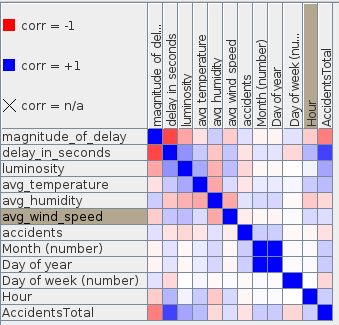
\includegraphics[width=0.5\linewidth]{Figures/correlationBraga.png}
    \caption{Correlação entre features após processamento.}
    \label{fig:corr1}
\end{figure}



